\chapter{State of the Art}
\label{chap:sota}
\begin{spacing}{1.5}
\sloppy
In the rapidly evolving landscape of artificial intelligence (AI), large language models (LLMs) have demonstrated remarkable results in text generation and understanding. Yet, when applied to real-world tasks such as question answering, these models still face significant limitations. As detailed in the previous chapter, LLMs are prone to hallucinations\footnote{In the context of LLMs, hallucinations refer to outputs that are plausible-sounding but factually incorrect, fabricated, or unsupported by the underlying data or external sources \citep{harsh_comprehending_2024}.}, rely on static and often outdated training data, and offer limited transparency or traceability in their outputs. Additionally, they may struggle to incorporate domain-specific context or organizational knowledge \citep{vaibhav_retrieval-augmented_2025}. These factors pose challenges for domains, like cultural heritage, GLAM and archaeology, where reliability, provenance, and interpretive rigor are fundamental requirements \citep{di_marcantonio_intelligenza_2024}.

To address these concerns, retrieval-augmented generation (RAG)\footnote{For more information about RAG technique, see \url{https://en.wikipedia.org/wiki/Retrieval-augmented_generation}.} has emerged as a crucial methodological advance. It improves the factual grounding and contextual relevance of generated answers, thorugh the integration of external and verifiable knowledge at inference time, thereby reducing the risk of generating fabricated or distorted information \citep{martineau_what_2023}. As discussed in \autoref{chap:QAS}, this approach represents a significant step beyond both traditional information retrieval and earlier neural QA models, which were often brittle, domain-dependent, or struggled to adapt to evolving information needs.
\sloppy
The adoption of RAG in question-answering reflects a broader evolution within the field: from early symbolic and rule-based systems, through statistical and information retrieval approaches, to today’s transformer-based, generative architectures. This shift has transformed not only the technical capabilities of QA systems but also their applicability to complex, heterogeneous knowledge domains.
\sloppy
Although initially developed for open-domain question answering and enterprise search \parencite{akkiraju_facts_2024, jiang_towards_2024, packowski_optimizing_2024, yang_ragva_2025, zhou_enabling_2025}, RAG pipelines are increasingly adopted in the humanities and cultural heritage contexts. In these sectors, where interpretive rigor, provenance, and information reliability are critical, RAG-based tools support scholars and professionals in navigating vast, fragmented knowledge repositories. While some initiatives employ RAG to analyze sensitive historical materials \citep{callaghan_prototyping_2025, ciletti_retrieval-augmented_2025, sergeev_talking_2025, fan_research_2025}, this thesis explores a distinct application: improving access to procedural and technical documentation, where clarity, consistency, and actionable guidance are the primary objectives.
\\

This chapter therefore provides a comprehensive overview of the state of the art in retrieval-augmented generation, situates RAG within the current research landscape, outlines its core mechanisms, and examines its recent application in the digital humanities.

\section{Core Mechanisms and Foundations of Retrieval-Augmented Generation}\setlength{\parskip}
{0pt}
Retrieval-augmented generation (RAG) is a hybrid approach designed to address several critical limitations of traditional LLMs, such as knowledge staleness, limited context awareness, and insufficient output traceability \parencite{vaibhav_retrieval-augmented_2025,gao_retrieval-augmented_2024, gupta_comprehensive_2024}. While LLMs excel at producing fluent, human-like text, they often falter when facing domain-specific queries or requests for information beyond their training cutoff. RAG directly addresses these challenges by integrating external information retrieval within the generation process, allowing outputs to be more factual, up-to-date, and grounded in verifiable sources \citep{wang_searching_2024}.

At its core, a typical RAG workflow consists of two main stages: \textbf{retrieval} and \textbf{generation} (\cite{odsc-community_retrieval-augmented_2024}). The process begins with preprocessing and indexing, where raw data is cleaned, extracted, segmented into manageable "chunks", and encoded into vector representations. These embeddings are then stored in a vector database (e.g., Milvus, Faiss, Qdrant)\footnote{Cf. glossary in \autoref{appendix:B}.} to facilitate efficient similarity searches. When a user submits a query, it is encoded in the same vector space, and the system retrieves the top-k most relevant chunks from the indexed knowledge base. In the subsequent stage, these retrieved documents are passed as context to a generative language model -- often based on Transformer architectures \citep{vaswani_attention_2017} -- which synthesizes a response that blends the original query with external evidence, producing answers that are both coherent and contextually appropriate \citep{arslan_survey_2024}.

This modular design (\autoref{fig:rag}) enables the continuous incorporation of domain-specific and current information, overcoming the constraints of static model parameters. Recent contributions have helped to formally systematize the RAG pipeline's, with frameworks delineating specific interdependent modules such as query classification, retrieval, re-ranking, and generation \parencite{wang_searching_2024,gao_retrieval-augmented_2024}.

\begin{figure}[H]
  \centering
  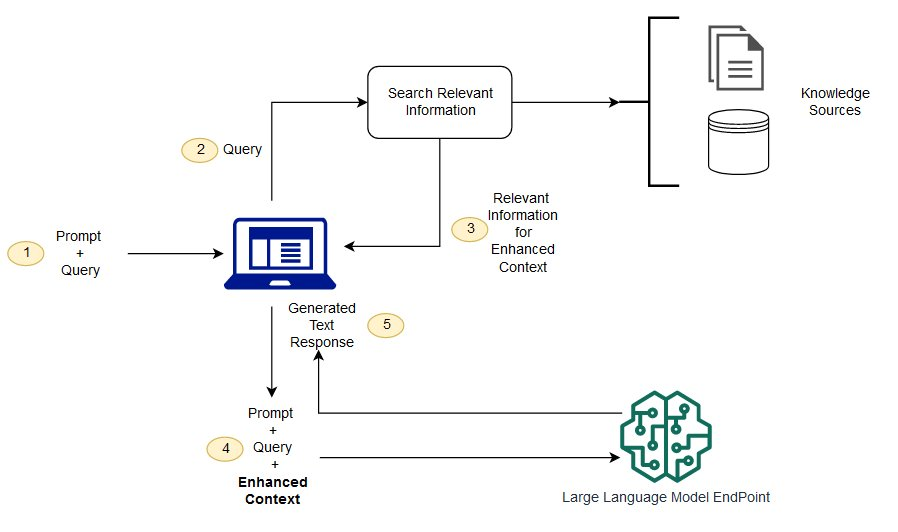
\includegraphics[width=\textwidth]{images/rag_workflow.jpg} 
  \caption{Typical RAG workflow.\\
  \footnotesize{Source: \url{https://aws.amazon.com/de/what-is/retrieval-augmented-generation/}.\nocite{noauthor_was_nodate}}}
  \label{fig:rag}
\end{figure}

\subsection{Pipeline Design and Common Practices}
The design of RAG pipelines can vary significantly based on the specific use case, domain, and available resources. However, several common practices have emerged that reflect the current state of the art in retrieval-augmented generation \citep{arslan_survey_2024, gupta_comprehensive_2024}.

The standard workflow includes the following components:
\begin{itemize}
  \item \textbf{Query understanding and classification:} Not all queries require retrieval from external sources. Advanced systems first analyse and classify incoming queries to determine whether retrieval is necessary or if the LLM alone suffices. This step leverages natural language understanding (NLU) techniques to extract key entities, relationships, and user intent, improving efficiency and reducing unnecessary retrieval latency.
  %Data Preparation and Indexing
    \item \textbf{Document indexing and chunking:} Raw data from source documents is preprocessed: cleaned, segmented into manageable "chunks" at token, sentence, or semantic level, and converted into dense vector representations (embeddings). Recent studies recommend dynamic or semantic chunking over simple fixed-size splitting, as it better preserves context and improves retrieval quality -- especially in heterogeneous domains.
    \item \textbf{Embedding and Vector Database:} Both document chunks and user queries are embedded into a shared vector space using models fine-tuned for semantic similarity (e.g., BAAI/bge, LLM-Embedder, intfloat/e5). These vectors are stored in efficient vector databases (e.g., Milvus, Faiss, Qdrant), selected based on scalability, indexing strategies, and support for hybrid (vector plus keyword) search capabilities.
    \item \textbf{Retrieval and query transformation:} Upon receiving a user query, the system encodes it into a vector and retrieves the top-k most relevant chunks from the indexed knowledge base (KB) using similarity search. Robustness is enhanced through hybrid retrieval, which combines dense (vector-based, e.g., DPR, Contriever) and sparse (lexical, e.g., BM25) methods. Advanced query transformation techniques -- including query rewriting, decomposition, or hypothetical document generation (e.g., HyDE)-- can further improve retrieval effectiveness.
    \item \textbf{Re-ranking:} Initially retrieved candidates are often re-ranked based on relevance to the original query, using additional models (DLM-based) -- e.g., cross-encoders like monoT5, monoBERT, or RankLLaMA, which jointly consider the query and each candidate -- or more sophisticated algorithms through heuristics. This contextualization ensures that the most pertinent information is prioritized for the generative model.\\See \autoref{tab:rerank_algorithms} for a summary on re-ranking techniques.
    \item \textbf{Repacking and summarization:} In some cases, retrieved passages may be reorganized or summarized to distill key information, especially when dealing with lengthy corpora. This step can involve extractive summarization or abstractive (e.g., with Pegasus or T5) techniques to condense information and fit within the context window of the generator model.
    \item \textbf{Generation:} The generative model -- usually a transformer-based LLM such as T5, BART, or GPT -- synthesizes a response conditioned on both the original query and the retrieved context, integrating intrinsic model knowledge with external evidence to produce a coherent, accurate, and contextually grounded answer.
\end{itemize}
\citep{vaibhav_retrieval-augmented_2025,wang_searching_2024,gao_retrieval-augmented_2024,gupta_comprehensive_2024}.


\begin{table}[H]
\centering
\footnotesize
\begin{tabularx}{\textwidth}{l X}
\toprule
\textbf{Algorithm} & \textbf{Rationale} \\
\midrule
Cross-Encoders & Joint encoding of query and document for fine-grained relevance scoring. \\
\cmidrule(lr){1-2}
TILDE \citep{zhuang_tilde_2021} & Token-level likelihoods for queries across a collection, allowing fast re-ranking by summing the probabilities of query tokens given each candidate passage. \\
\cmidrule(lr){1-2}
Learning-to-Rank (LTR \citep{gupta_comprehensive_2024}) & Traditional machine learning ranking approaches: \textbf{a) Pointwise:} predicts relevance score for each document independently; \textbf{b) Pairwise:} compares pairs of documents to learn relative relevance; \textbf{c) Listwise:} considers the entire ranked list at once.\\
\cmidrule(lr){1-2}
Hybrid sparse + dense scoring & Blends scores from dense retrievers (semantic similarity -- e.g., DPR, Contriever) and sparse methods (lexical overlap -- e.g., BM25, TF-IDF) for robust ranking. Sometimes uses learnable weighting \citep{wang_searching_2024}. \\
\cmidrule(lr){1-2}
Graph-based \citep{han_retrieval-augmented_2025} & Constructs a graph of candidates (nodes) based on relationships (semantic, citation, or knowledge graph edges), then uses graph algorithms  (e.g., PageRank, label propagation) to identify central passages. \\
\cmidrule(lr){1-2}
Self-RAG (LLM-enhanced reranking) \citep{asai_self-rag_2023} & Uses LLMs directly to score or select the most relevant passages, sometimes via few-shot prompting or chain-of-thought reasoning. \\
\bottomrule
\end{tabularx}
\vspace{0.5em}
\caption{Algorithms for document re-ranking in RAG pipelines.}
\label{tab:rerank_algorithms}
\end{table}

\subsection{Evaluation and Benchmarking}
Evaluating RAG systems poses unique challenges, as traditional metrics like BLEU or ROUGE may not fully capture the quality of generated responses, particularly regarding factual accuracy and contextual relevance. To address these shortcomings, researchers have introduced specialized benchmarks and frameworks. For example, the Retrieval-Augmented Generation Assessment System (RAGAS) specifically targets the evaluation of answer faithfulness and contextual alignment, offering a more nuanced perspective on RAG system performance \citep{es_ragas_2023}. Human-in-the-loop evaluations have also gained prominence, with expert judges assessing generated responses on criteria such as coherence, factual accuracy, and relevance to original queries -- providing richer and more reliable quality assessments than automated metrics alone \citep{gupta_comprehensive_2024}.

Continuous evaluation against established benchmarks like BEIR \citep{thakur_beir_2021} and TREC \citep{voorhees_trec_2005} remains essential for tracking performance across diverse retrieval and generation tasks. Regular benchmarking ensures that systems maintain high standards for accuracy, relevance, and user satisfaction. Even after deployment, proactive monitoring is critical. Tracking system performance, user interactions, and error patterns allows teams to address issues quickly and keep RAG solutions reliable and effective as data and usage patterns evolve \citep{amershi_software_2019}.

Ethical considerations must be embedded throughout the lifecycle of RAG systems. Prioritizing data privacy, addressing algorithmic bias, and complying with regulations such as GDPR are fundamental. This involves designing systems for transparency, explainability, and responsible AI use, as well as ongoing audits to ensure ethical standards are met \citep{jobin_global_2019}.

The trajectory of RAG systems points toward increasingly sophisticated applications that are deeply integrated into the workflows of research, industry, and cultural institutions. Innovations in evaluation frameworks, user interaction, and system scalability are steadily pushing the boundaries of what these models can achieve. As these technologies continue to mature, success will depend on the ability to combine robust benchmarking, user-centered feedback mechanisms, and adaptive optimization strategies. Addressing challenges related to factuality, scalability, and responsible deployment will be essential for building trustworthy systems capable of delivering high-quality, contextually relevant information. With continued progress, RAG systems are set to play a pivotal role in shaping the future of digital knowledge access and discovery. \parencite{wang_searching_2024, gao_retrieval-augmented_2024}.

\section{New Frontiers Applications}\label{sec:evol_qas}
RAG systems are increasingly deployed across diverse domains -- spanning academia, enterprise, and product environments -- to enhance data accessibility, support decision-making, and facilitate natural language interaction with complex knowledge bases. Recent surveys and empirical studies document a growing array of scholarly applications of RAG, including:
\begin{itemize}
    \item Automated literature review tools and citation management -- e.g., LitLLM; \citep{agarwal_litllm_2025}, KNIMEZoBot; \citep{alshammari_knimezobot_2023};
    \item Generation of summaries for large corpora of academic papers;
    \item Field-specific knowledge extraction, including biomedical and legal research support.
\end{itemize}

\noindent In one experiment, a RAG system was developed to assist data scientists through a combination of GROBID library\footnote{GROBID is a machine learning library designed to extract, parse, and convert raw documents, like PDFs, structured XML/TEI encoded documents \citep{GROBID}.} for structured bibliographic extraction, fine-tuned embeddings, semantic chunking, and an abstract-first retrieval strategy. The system's performance, assessed using the Retrieval-augmented generation Assessment System (RAGAS), demonstrated improved faithfulness and context relevance in response generation \citep{aytar_retrieval-augmented_2024}. A similar approach was explored in the context of academic library systems, where RAG was applied to improve contextual retrieval through semantic indexing of structured metadata (e.g., MARC/RDA standards) and multimodal resources. Additionally, the framework introduced conversational querying via a natural language interface, supporting complex interdisciplinary searches and significantly improving document discoverability by synthesizing citation-backed responses from diverse scholarly sources -- including journals, datasets, and videos. This solution also addressed challenges such as copyright compliance and ethical AI transparency \citep{bevara_prospects_2025}.  Collectively, these studies affirm RAG systems’ efficacy in alleviating information overload and improving research workflow discoverability.

In parallel, the work of \citep{soman_observations_2024} provides further critical insights into the design of RAG systems for domain-specific and technical content, closely aligning with the methodological framework adopted in the GNA question-answering system. Using IEEE telecommunications engineering corpora (i.e., wireless LAN specifications and battery glossaries) as testbeds, their analysis highlights key factors influencing retrieval quality, which include chunk size, sentence-level similarity, and the strategic placement of domain-specific terms. These aspects are similarly addressed in the GNA RAG pipeline \citep{pograri_question-answering_2025}, which applies customized tailored chunking, semantic preprocessing, and contextual embedding strategies. Both studies advocate for more nuanced, context-aware approaches to enhance precision in technical and highly structured domains.

Numerous recent graduate-level research projects have provided substantive input into the implementation and evaluation of RAG systems:
\begin{itemize}
    \item \textcite{antolini_experimental_2025} developed a custom RAG system for open-domain question answering using both traditional (BM25, PRF) and advanced retrieval strategies, integrated with local LLMs. A novel Parametric RAG (PRAG) approach was also explored, embedding context into model parameters for performance gains.
    \item \textcite{caramanna_progettazione_2024} investigated conversational agent architectures, comparing various LLM types and retrieval configurations.
    \item \textcite{florio_progettazione_2024} implemented a LangChain-based RAG chatbot for corporate documentation, evaluating multiple vector database technologies.
    \item \textcite{salcuni_utilizzo_2025} applied RAG to the medical domain, improving LLM responses in hypertension care. The study used RAGAS to assess quality and relevance, focusing on personalization and accuracy.
    \item \textcite{nicoletti_llms_2025} developed Essence Coach, a chatbot that integrates LLMs with the Essence software engineering standard. This system significantly outperformed generic LLMs like GPT-4o in domain-specific reasoning tasks.
\end{itemize}

\section{RAG in the Digital Humanities}\label{sec:rag_dh}
A growing body of research is exploring RAG applications within the digital humanities. One such example is the \textit{iREAL} project, which applied RAG to interpret archival records from Aboriginal schools in Australia, demonstrating a careful balance between cultural sensitivity and historical accuracy \citep{callaghan_prototyping_2025}. Another initiative, \textit{ValuesRAG}, focuses on cultural alignment in LLMs by integrating societal and demographic knowledge through retrieval-augmented contextual learning, experimenting with the \textit{World Values Survey} dataset \citep{seo_valuesrag_2025}. In another case, the \textit{Foggia Occupator Dataset} project applied a RAG model to post-WWII Italian periodicals, extracting information on political figures and stylistic traits \citep{ciletti_retrieval-augmented_2025}.

Among the technical approaches explored in recent experiments on generative AI for digital scholarly editions, RAG emerges as a promising method for addressing challenges such as entity linking (EL) and the integration of external knowledge sources. Notably, RAG is recognized for its ability to mitigate hallucinations in named entity recognition (NER) and to enable the enrichment of text with information from structured databases or knowledge graphs \citep{pollin_when_2025}. For example, the \textit{Regesta Imperii} project demonstrates how knowledge bases, including Neo4j graph databases, are leveraged within RAG pipelines to improve accuracy in information extraction, entity normalization, and semantic annotation \citep{kuczera_chatgpt_2024}. Similarly, the editorial workflow developed for the \href{https://web.archive.org/web/20241120122545/https://gams.uni-graz.at/context:hsa}{Hugo Schuchardt Archive} outlines a process that combines prompt engineering, human-in-the-loop oversight, and RAG-enabled toolchains to enhance the generation of TEI-compliant XML, supporting more explainable and modular processing pipelines \citep{pollin_new_2023}. These and other experiments underscore the need for standardized workflows, robust evaluation protocols, and systematic research into both the strengths and weaknesses of LLMs and related tools in the editorial process, while also advocating for thoughtful engagement with advanced computational methods in the humanities \citep{pollin_workshop_2024}. As digital editions become increasingly complex and interconnected with broader knowledge infrastructures, the relevance and application of AI technologies -- such as RAG -- are both expected and desirable to grow accordingly.

RAG methodologies are being adopted within the GLAM sector (Galleries, Libraries, Archives and Museums) as well. In archival contexts, a smart assistant developed for querying the \textit{Prozhito} digital archive of personal diaries combines text-to-SQL filtering, hybrid search, and automatic query reformulation, proving especially effective for historians and anthropologists without prior knowledge of database query languages  \citep{sergeev_talking_2025}. Meanwhile, in museum settings, a comparative evaluation of RAG systems versus large-context LLMs for answering multimodal questions about artworks demonstrated that the RAG approach offers superior precision and explainability \citep{ramos-varela_context_2025}.

Innovations in graph-based retrieval are also gaining momentum. Techniques combining structured supervision and chain-of-thought prompting have been used to map character relationships in early modern English historiography, thereby reducing the manual workload typically associated with historical data annotation \citep{fan_research_2025}. Related directions are being explored within cultural heritage institutions, as seen in the \textit{CAT-IA} initiative \citep{barbato_nasce_2025}, which integrates ArCo knowledge graph \citep{carriero_arco_2019} within a RAG system for provenance tracking, AI explainability (XAI), and structured metadata extraction. Designed to streamline and enrich user interactions with the General Catalogue of Cultural Heritage \textit{(Catalogo generale dei beni culturali)}, \textit{CAT-IA} marks a notable stride in applying advanced digital technologies to promote accessibility and valorization of cultural assets.

A complementary, conceptual perspective emerges in a critical mapping of the theoretical contours of RAG within the broader landscape of archives, libraries, and cultural heritage -- articulating not only the potential for RAG-augmented LLMs to enhance the precision, accessibility, and contextualization of information retrieval, but also foregrounding the social and infrastructural challenges inherent in such integration. This analysis is accompanied by a caution against viewing RAG as a substitute for established cataloguing practices. This viewpoint encourages the field to reflect on both the affordances and the epistemic and ethical complexities introduced by RAG systems in digital humanities contexts \citep{di_marcantonio_intelligenza_2024}.


Finally, efforts to advance access to fragmented digital repositories -- such as web archives -- have increasingly adopted RAG methodologies. An illustrative bespoke prototype \citep{davis_unlocking_2025} transforms keyword-based search into semantically guided question answering, sharing architectural parallels with the GNA QA system presented in the context of this thesis. Both systems prioritize semantic retrieval over lexical matching using dense embeddings -- e.g., \textit{E5} variants \citep{wang_text_2024} -- to interpret queries in context, employ structured text processing pipelines to reduce noise in source materials, and apply optimized chunking strategies for retrieval accuracy. Crucially, these studies highlight RAG’s potential to transform scattered and heterogeneous resources -- whether web archives or catalographic procedures -- into coherent, accessible knowledge through context-aware synthesis.

\section{Future Directions}
Ongoing research is rapidly pushing the frontiers of RAG, opening up new avenues  that extend well beyond traditional information retrieval into domains such as scientific research and the digital humanities. Among the most promising innovations is the use of synthetic corpora to bolster the robustness and generalizability of RAG systems, particularly in low-resource or specialized domains where annotated data is scarce \citep{bor-woei_generative_2024}. This strategy not only improves retrieval accuracy but also addresses longstanding issues of bias, coverage, and representativity in humanities corpora. 

RAG is also at the core of a new wave of applications that automate and enhance scholarly practices. In scientific research, advanced RAG frameworks -- including agentic systems like PaperQA \citep{lala_paperqa_2023}-- are being leveraged to conduct systematic literature reviews, automate evidence synthesis, summarize emerging trends, and provide transparent citation recommendations. These multi-stage agentic architectures enable recursive reasoning, dynamic tool use, and context-aware synthesis, often surpassing human-level performance in both retrieval and summary tasks. Their capacity for rigorous, scalable analysis offers substantial promise for the digital humanities as well, facilitating the synthesis of dispersed cultural resources and supporting complex, interpretive scholarly inquiries \citep{skarlinski_language_2024}.

Despite these advances, several critical research challenges remain. There is an urgent need to develop domain-adapted and multilingual LLMs that can process not just text, but also multimodal data such as images, tables, and audiovisual materials—a key requirement for both scientific and cultural heritage applications. Future RAG systems should be able to retrieve and reason over heterogeneous, cross-domain sources, necessitating robust mechanisms for source evaluation, multimodal fusion, and trust calibration. The ongoing development of benchmarks and evaluation datasets, tailored to the nuanced needs of fields such as the digital humanities, is essential to guide progress and ensure methodological rigor \citep{yue_survey_2025}.

Another major direction is the semantic enrichment of RAG pipelines through the integration of ontologies and knowledge graphs. Ontologies, as formal domain knowledge models, provide structured frameworks that enable more precise and explainable retrieval semantic coherence, and the inclusion of ethical dimensions in generative AI. Complementing this, knowledge graphs capture complex relationships and support context-aware multi-hop reasoning, improving accuracy, explainability, and cultural sensitivity of outputs. Current research and practical applications span a range of initiatives – from ontology-guided entity typing to the grounding of AI in explicit ethical and procedural knowledge, demonstrating that these semantic tools are essential for creating robust, context-aware, and transparent RAG systems, addressing challenges in fields as diverse as healthcare, engineering, scientific discovery, and enterprise knowledge management \citep{tiwari_ontorag_2025, ludwig_ontology-based_2025, bran_ontology-retrieval_2024, sharma_og-rag_2024, xiao_orag_2024, park_ontology-based_2024, debellis_integrating_2024,franco_ontology-based_2020}.

In the specific context of the digital humanities, the accelerated adoption of AI is shaping a transformative future for scholarship, curation, and access to cultural heritage. The diverse case studies and technical innovations, discussed in \autoref{sec:rag_dh}, illustrate both the breadth of RAG’s impact and the field’s growing ambition. Across applications, from digital scholarly editions, to archival assistance and museum information systems, RAG has is emerging as a pivotal enabler for addressing the limitations of traditional search and annotation by supporting context-aware, semantically rich, and explainable information access.

Looking forward, several converging trends and open challenges will define the evolution of RAG in the digital humanities. First, technical advances such as the integration of knowledge graphs, graph-based retrieval, and multimodal pipelines are driving improvements in improving semantic linking and annotation of historical, literary, and artistic materials. Second, the increasing complexity of digital scholarly editions and GLAM infrastructures is catalyzing demand for standardized, reproducible workflows, robust evaluation protocols, and domain-adapted benchmarks, ensuring that RAG methods are critically assessed and tuned for the nuanced needs of humanistic research.

At the same time, as digital repositories become ever more fragmented, the promise of RAG lies in its ability to synthesize heterogeneous, dispersed data -- transforming scattered web archives, periodicals, and catalogues into accessible, contextualized knowledge spaces. Yet, this evolution also foregrounds critical conceptual and ethical questions. As highlighted by recent critical perspectives, it is essential to position RAG as an augmentative technology: one that enhances, but does not replace, established cataloguing, metadata, and interpretive practices. human interpretive oversight, transparency, and cultural sensitivity must remain central, particularly as RAG systems are increasingly relied upon for knowledge production and mediation in complex social and historical domains \citep{di_marcantonio_intelligenza_2024}.

In sum, the next phase of RAG’s development in the digital humanities will require sustained interdisciplinary collaboration and critical reflection. Researchers and practitioners must continue to experiment with new strategies, but also engage deeply with the epistemic, social, and infrastructural complexities of integrating advanced AI into cultural knowledge management. Ultimately, RAG applications stand poised not only to offer improved access to information, but they also invite a reimagining of the relationship between artificial intelligence and cultural knowledge production, fostering tools that augment – not displace – human creativity and understanding.
\end{spacing}